\chapter{Implementácia}
Firmvér senzorovej jednotky je implementovaný v programovacom jazyku C s hardvérovými ovládačmi poskytovanými
SDK Espressif IoT Development Framework. Súbežný beh úloh spravuje operačný čas reálneho času FreeRTOS.
Optimalizované rutiny digitálneho spracovania signálu zahŕňa Espressif DSP Library. Knižnica MPack má na starosti
kódovanie a dekódovanie formátu Message Pack. Nástroj na automatizáciu kompilácie CMake riadi zostavovanie modulov zdrojového
kódu. Eclipse Mosquitto pôsobí ako MQTT broker správ.

V jazyku Python sú napísané Jupyter notebooky na analýzu zozbieraných datasetov a otestovanie fáz navrhnutej dátovej pipeline.
s balíčkami numpy, scipy, pandas a matplotlib. Rozhranie príkazového riadku na nahrávanie konfigurácie a náhľad odoberaných
správ sa spolieha na externé balíčky Paho MQTT, cmd a msgpack. Návod na inštaláciu a konkrétne verzie sú uvedené v prílohe

\begin{figure}[h]
\centering
\begin{subfigure}[b]{0.6\textwidth}
    \centering
    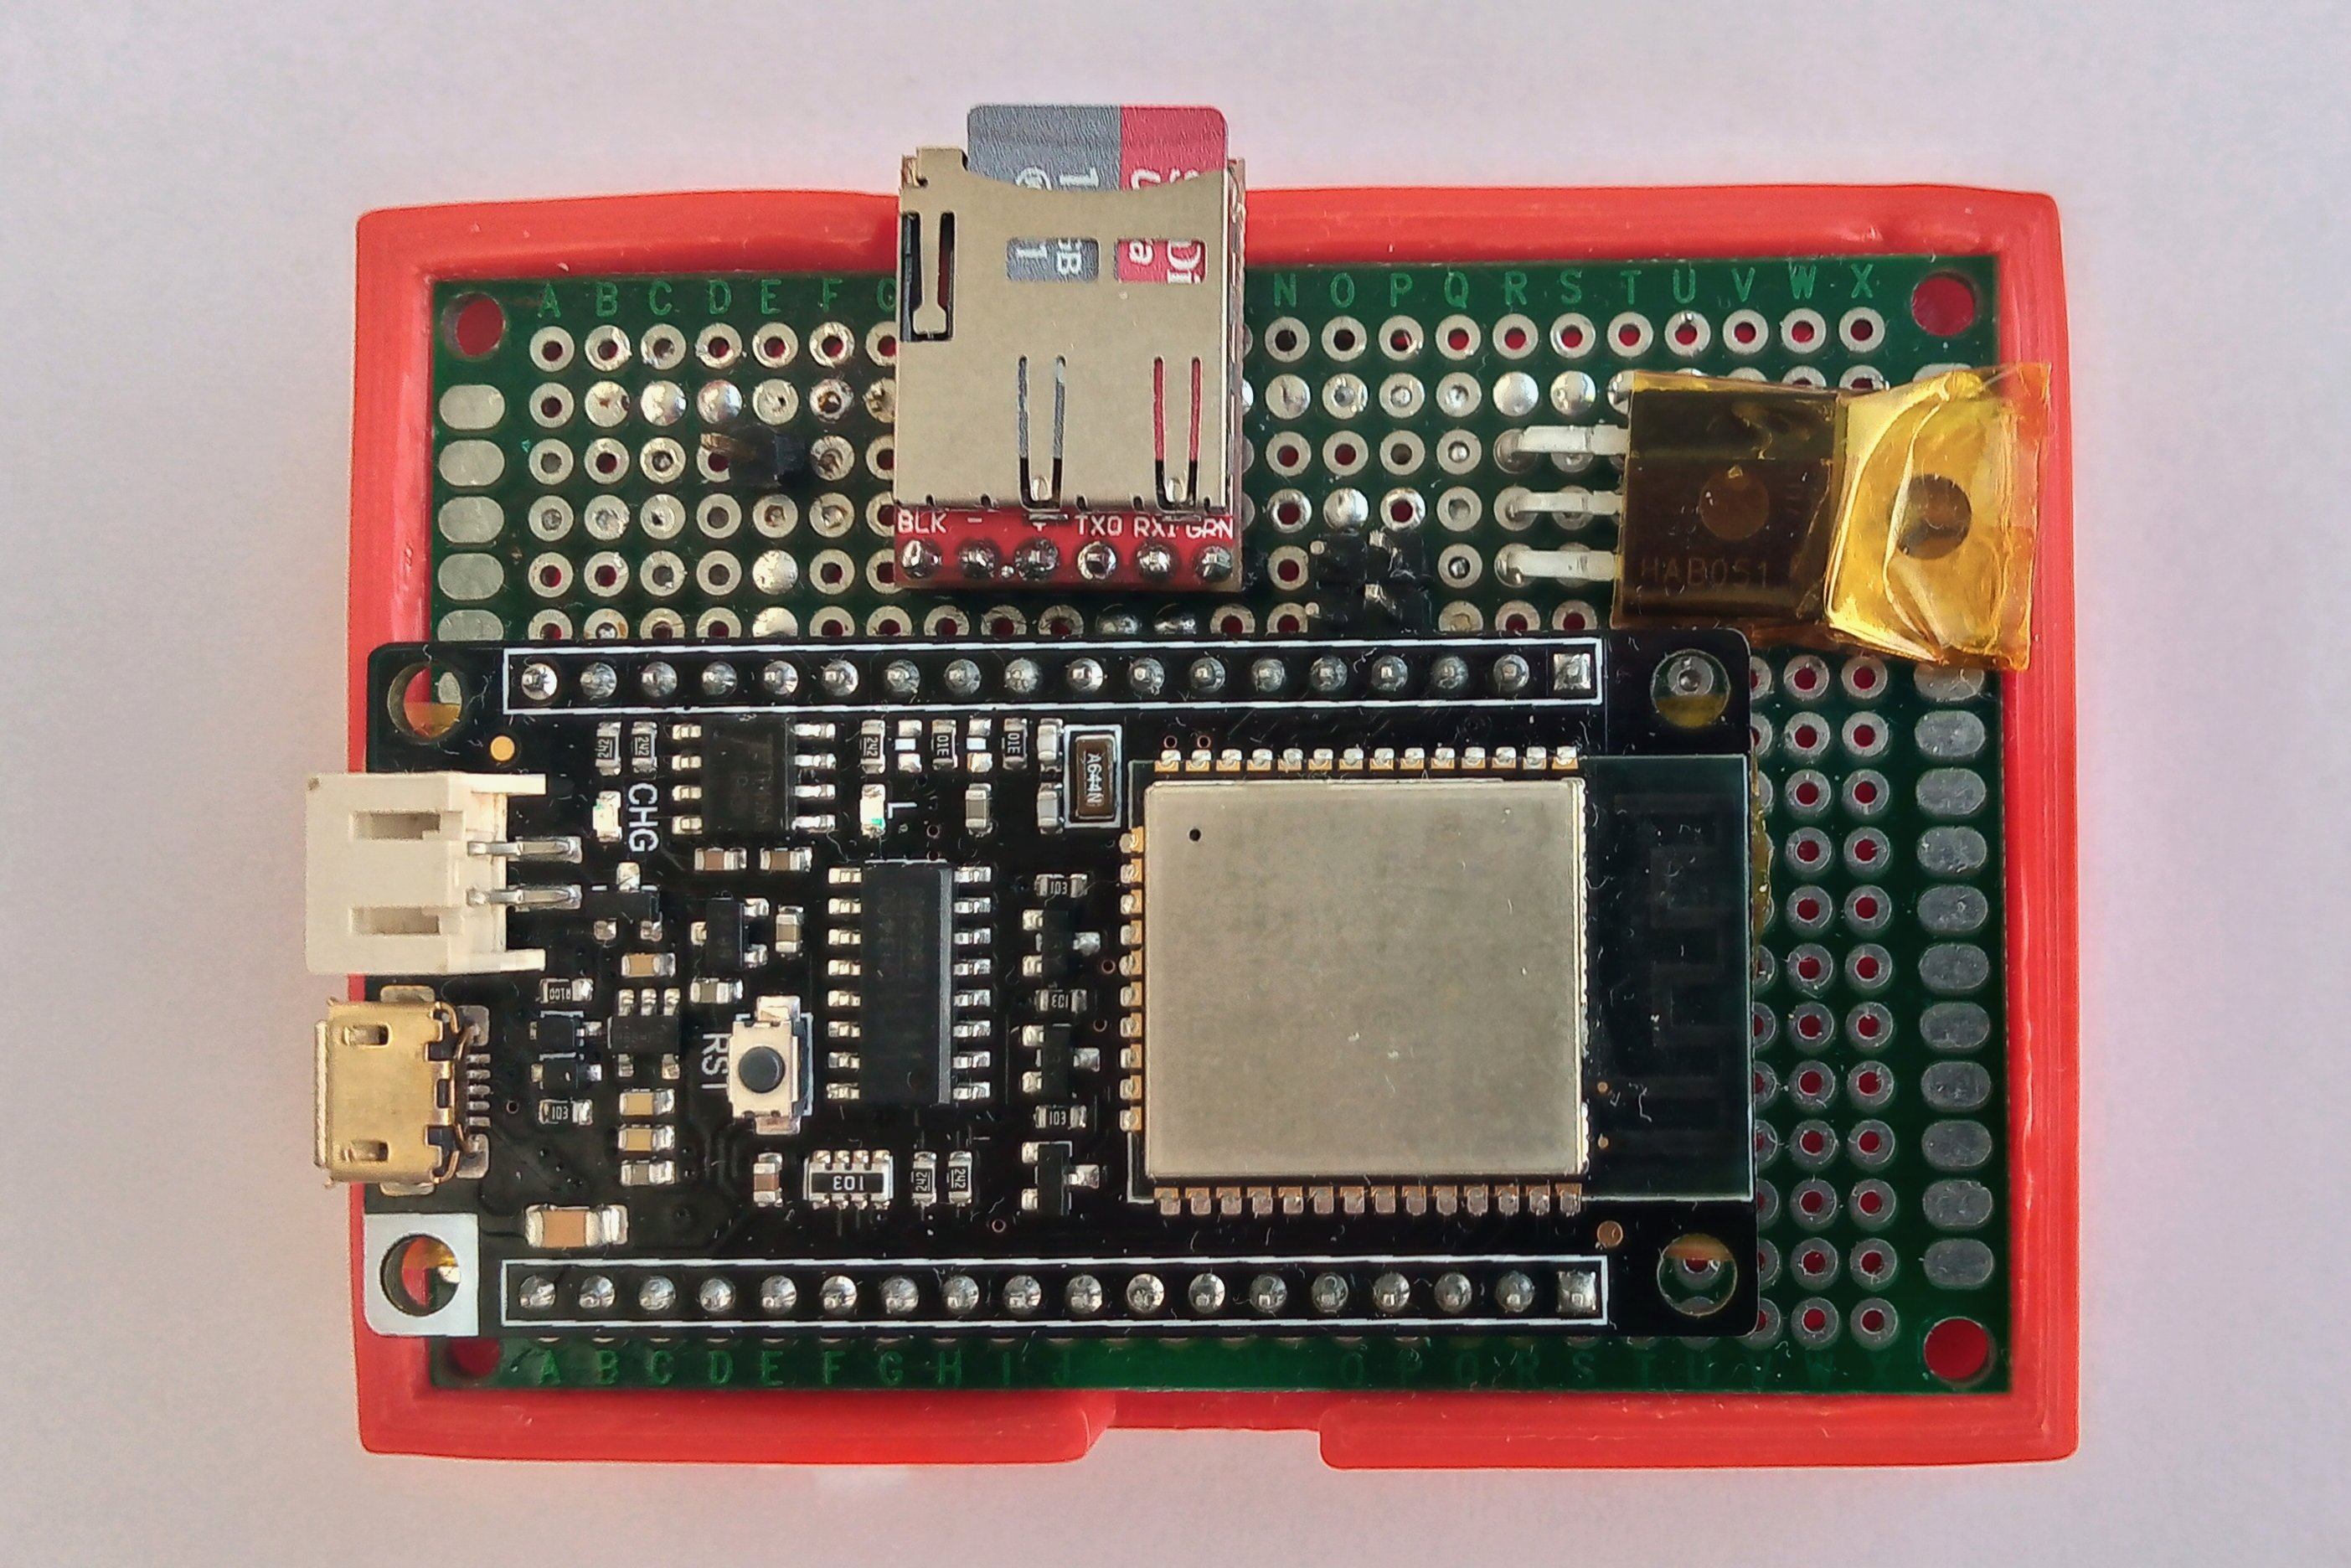
\includegraphics[width=\textwidth]{figures/design/esp32.jpg}
\end{subfigure}
\begin{subfigure}[b]{0.2\textwidth}
    \centering
    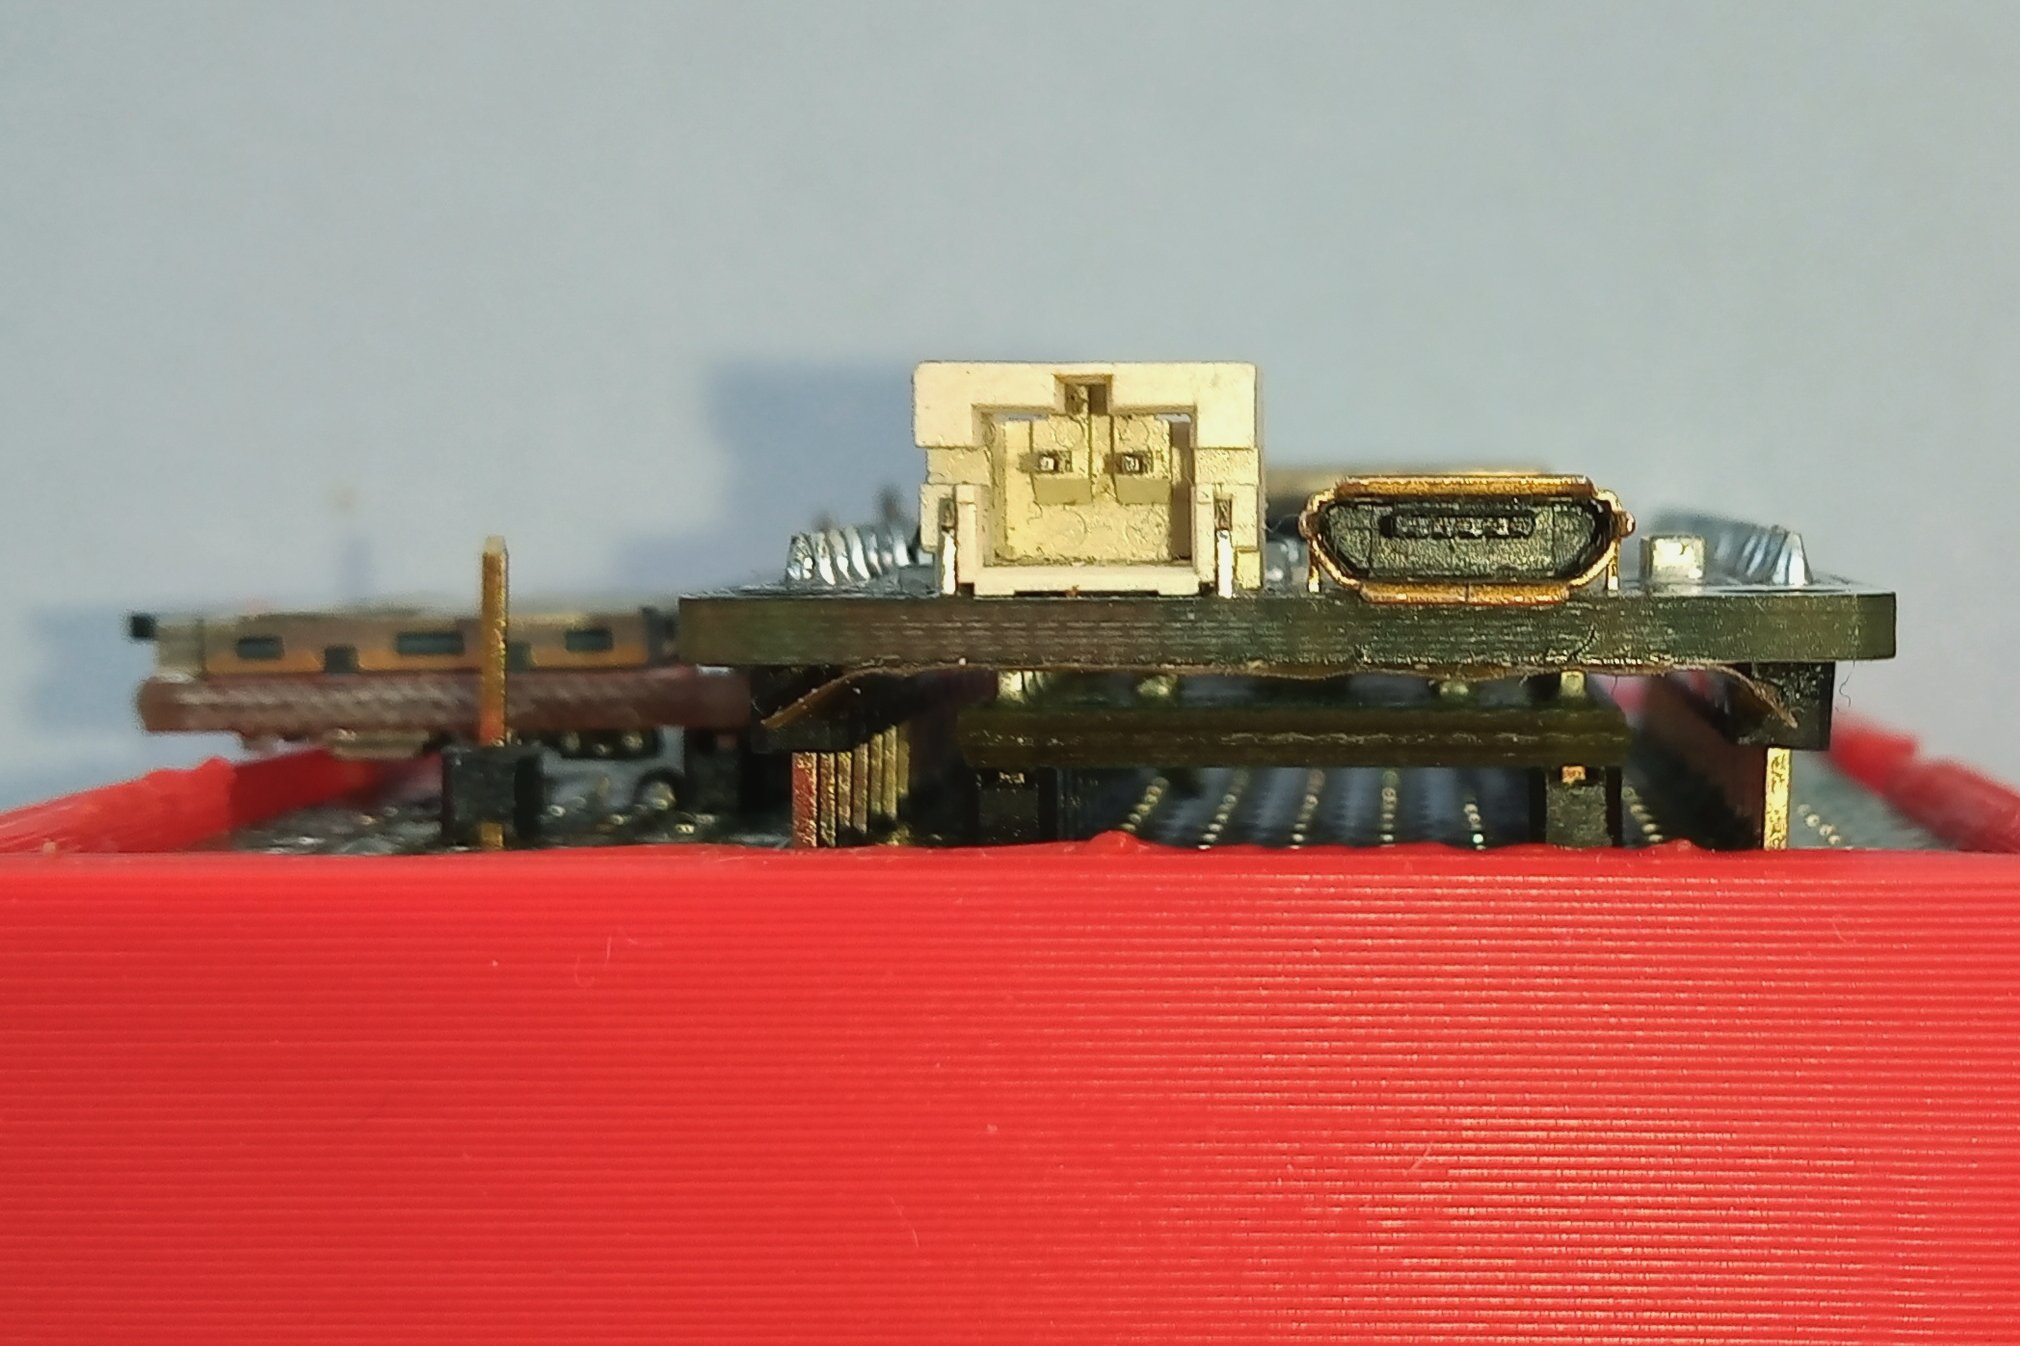
\includegraphics[width=0.9\textwidth]{figures/design/esp32-front.jpg}
\end{subfigure}
\caption{Univerzálny plošný spoj v krabičke osadený modulmi}
\label{board}
\end{figure}

\section{Senzorová jednotka}
Súčiastky FireBeetle ESP32, OpenLog, STEVAL-MKI159V1 a BTS117 sú naspájkované na univerzálny plošný spoj rozmerov 5 x 7 cm 
(obr. \ref{board}). Doska je vsadená na plastovej krabičky s hrúbkou stien 3 mm vo výške 2 cm nad povrchom. Akcelerometer je namontovaný 
tesne pod modulom MCU. Externý 5 V zdroj sa pripája cez Micro USB konektor, alebo cez JST PH 2 pin zapojíme 3,7 V lítiovú batériu.

\section{Komunikácia medzi úlohami}
Nezávislé činnosti aplikácie sú prerozdelené medzi vlákna, ktoré si cez fronty posielajú súradnice zrýchlenia.
FreeRTOS úlohy sú funkcie vykonávajúce opakované sekvenciu príkazov v nekonečnom cykle. 

Procedúra obsluhy prerušenia časovača nesmie čakať, preto je načítaná rovno z IRAM a upovedomí úlohu vzorkovania (kód \ref{lst:sampling}). 
Prevzatím notifikácie synchrónne pošle riadiace slovo senzoru na sekvenčné odčítanie celého vektora akcelerácie od bázovej adresy
registra x-ovej osi. Získaná trojica 16-bitových slov sa podľa aktuálneho rozlíšenia prevedie do štandardnej fyzikálnej jednotky
v type \verb|float|.

\begin{lstlisting}[style=cstyle,caption=Posielanie vzoriek medzi úlohami cez fronty,label={lst:sampling},
 morekeywords={ulTaskNotifyTake,xQueueSend,xQueueReceive}]
// Sampling task
if (ulTaskNotifyTake(pdTRUE, portMAX_DELAY)) {
	imu_acceleration(&imu, &axis[0], &axis[1], &axis[2]);
	for (i = 0; i < AXIS_COUNT; i++) {
    	if (conf.sensor.axis[i])  
        	xQueueSend(pipeline.queue[i], &axis[i], 0);
    }
}
// Pipeline task
if (xQueueReceive(k->queue[x], &p.stream[idx], portMAX_DELAY)) {
	if (++idx < conf.sensor.n) continue;
    // Process buffer
    buffer_shift_left(p.stream, conf.sensor.n, leftover);
    idx = conf.sensor.n - leftover;
}
\end{lstlisting}
Vkladanie vzoriek do fronty neblokuje, lebo sa nepočíta s úplným vyčerpaním voľných slotov. Zároveň
sa cez frontu posiela iba vtedy, ak beží úloha pipeline pre danú dimenziu. Na opačnom konci fronty opúšťajúce čísla 
sa po jednom pripájajú do cirkulárnej vyrovnávacej pamäte. 

Pole sa prenechá zvyšku úlohy na spracovanie po vyčerpaní vyhradeného priestoru podľa
systémovej konfigurácie \verb|conf.sensor.n|. Dokončením analýzy posuvného okna sa presunú ponechané hodnoty tvoriace prekryv časových 
úsekov na začiatok poľa: $\mathrm{leftover} = n \cdot (1 - \mathrm{overlap})$. 
Ďalej sa pokračuje prepisovaním už nepotrebných čísel od pozície \verb|idx|.

\begin{lstlisting}[style=cstyle,caption=Synchronizácia úloh na výpočet korelácie osí,label={lst:correlation},
morekeywords={xEventGroupSync}]
xEventGroupSync(barrier, (1 << axis), task_mask, portMAX_DELAY);
	float avg = mean(buffer, n);
	std[axis] = sqrt(variance(buffer, n, avg));
	for (uint16_t i = 0; i < n; i++)
		diff[axis][i] = (buffer[i] - avg);
xEventGroupSync(barrier, (1 << axis), task_mask, portMAX_DELAY);

if (axis[0] && axis[1])
   stats->corr_xy = correlation(diff[0], diff[1], n, std[0], std[1]);
\end{lstlisting}

Okrem synchronizácie úloh frontami na posielanie správ sa zužitkúvajú bariéry. Event Groups riadia toky 
synchronizovaných úloh v bodoch stretu čakaním na nastavenie bitov podľa očakávanej bitovej masky. Počas
autorizácie voči prístupovému bodu WiFi čaká podprogram hlavného vlákna na príznak pridelenia IP adresy
od obsluhy udalosti nadviazania spojenia. 

Koordinácia vlákien je nevyhnutná tiež pri výpočte korelácie, pretože každá os sa rieši nezávisle. Proces prezentuje zjednodušený
kód \ref{lst:correlation}.V sekcii medzi bariérami si úlohy predpočítajú smerodajnú odchýlku a zoznam rozdielov 
od aritmetického priemeru. Konštanta \verb|task_mask| značí bitovými vlajkami, ktoré osi sú aktivované. 
Na základe $\mathrm{axis} \in \{0,1,2\}$ signalizuje konkrétne vlákno, že prišlo ku bariére. Mimo kritickej oblasti 
si jednotlivé vlákna disponujúce medzivýsledkami za každú zložku vektora dorátajú individuálne momentálne povolené 
kombinácie dvojíc.

\section{Frekvenčná transformácia}
Uprava DCT v knižnici
\begin{lstlisting}[style=cstyle,caption=Transformácia do frekvenčnej domény]
for (uint16_t i = 0; i < n; i++) {
	spectrum[2*i+0] = buffer[i] * window[i]; 
	spectrum[2*i+1] = 0;
}
dsps_fft2r_fc32_ae32(spectrum, n);
dsps_bit_rev2r_fc32(spectrum, n);
dsps_cplx2reC_fc32(spectrum, n);
\end{lstlisting}
 
Magnituda spektra v dB
\begin{lstlisting} [style=cstyle]         
for (uint16_t i = 0; i < bins; i++)
	spectrum[i] = dsps_sqrtf_f32_ansi(
          square(spectrum[i*2]) + square(spectrum[i*2+1])
    );

float ref = maximum(spectrum, bins);
for (uint16_t i = 0; i < bins; i++)
	spectrum[i] = 20 * log10f(spectrum[i] / ref);
\end{lstlisting}


\section{Detekcia udalostí}
\begin{lstlisting}[style=cstyle]
typedef struct {
    SpectrumEventAction action;
    uint32_t start;
    uint32_t duration;
    int32_t last_seen;
    float amplitude;
} SpectrumEvent;
\end{lstlisting}

\section{Vzdialená konfigurácia}
- Nástroj klienta
- Opis štruktúr konfigurácie
- Uloženie v pamäti
\begin{lstlisting}[style=cstyle]
typedef struct {
    SamplingConfig sensor;
    SmoothingConfig tsmooth;
    StatisticsConfig stats;
    FFTTransformConfig transform;
    SmoothingConfig fsmooth;
    EventDetectionConfig peak;
    SaveFormatConfig logger;
} Configuration;
\end{lstlisting}

\begin{verbatim}
# /etc/mosquitto/mosquitto.conf
listener 1883 0.0.0.0
allow_anonymous true
\end{verbatim}

\emptypage
